\subsection{Poster Session 6}

This poster session contained quite some papers related to the medicine.
Self-supervision seem to be the general trend these days.


\spacerule
\subsubsection{Differentiable Augmentation for Data-Efficient GAN Training \cite{ZhaoLLZ020}}

Presented by \textit{Shengyu Zhao} \\

{\bf Motivation:} collecting datasets is expensive. 
However, GANs trained on limited datasets suffer from low performance because it becomes easier for discriminator $D$ to just memorize training set (overfitting). Figure \ref{fig:gan_overfitting_on_limited_data} illustrates this phenomena. \\

\begin{figure}[h!]
    \centering
    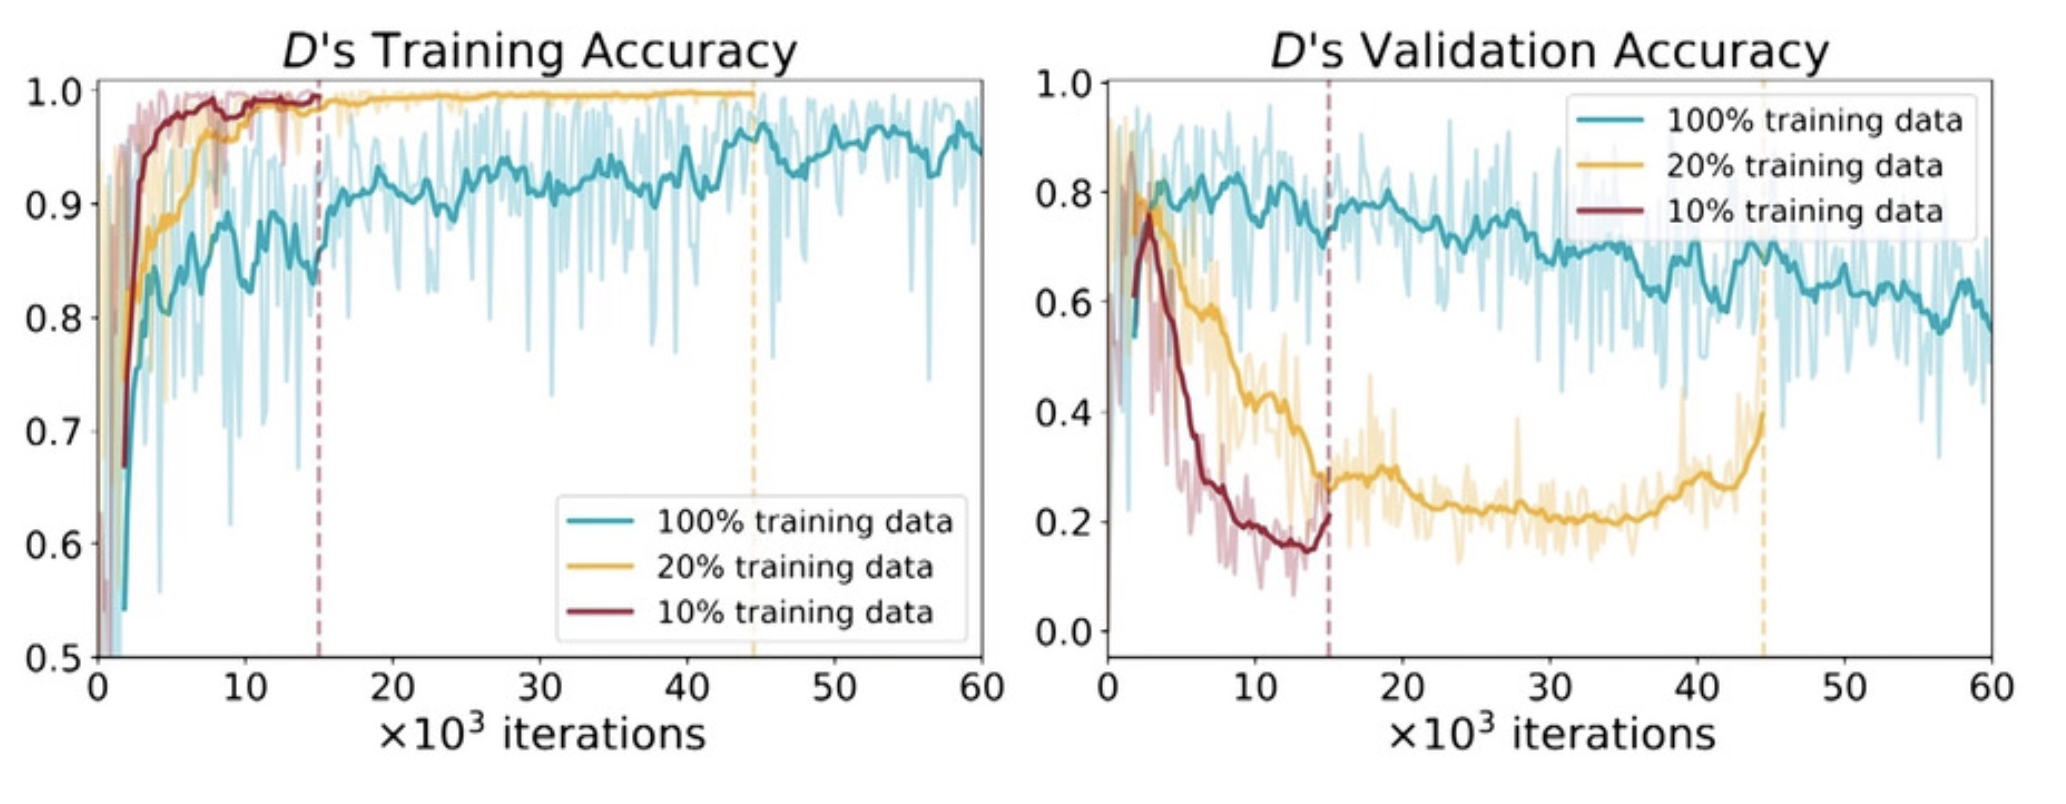
\includegraphics[scale=0.4]{neurips-2020/images/Screenshot 2020-12-11 at 10.29.55.png}
    \caption{Accuracy of the discriminator $D$ model rapidly increases when number of training samples becomes smaller. In the 20\% case training accuracy rapidly saturates while validation accuracy keeps decreasing until collapse. This phenomenon becomes more severe with only 10\% of data available.}
    \label{fig:gan_overfitting_on_limited_data}
\end{figure} \\

{\bf Observation:} data augmentation can increase variability of data in case of limited datasets. \\

{\bf Problems:}
\begin{itemize}
    \item if augmentations are only introduced to the real images, outputs generated by the generator $G$ will suffer from artefacts similar to the used augmentations
    \item if augmentations are introduced to both real and fake images but used only to train $D$, it leads to even worse results because $G$ and $D$ now are trained for different tasks
\end{itemize} \\

{\bf Proposal:} introduce differentiable augmentations to modify real and fake images for both $G$ and $D$. Consider the following basic GAN definition (equation \ref{eq:gan_eq}):

\begin{equation}
  \begin{array}{l}
    L_D = \mathbb{E}_{\pmb{x} \sim p_{data}(\pmb{x})} [f_D(-D(\pmb{x}))] + \mathbb{E}_{\pmb{z} \sim p(\pmb{z})} [f_D(D(G(\pmb{z})))] \\
    \\
    L_G = \mathbb{E}_{\pmb{z} \sim p(\pmb{z})} [f_G(-D(G(\pmb{z})]
  \end{array}
  \label{eq:gan_eq}
\end{equation}

Equation \ref{eq:gan_eq} is changed to introduce differentiable augmentation $T$ as a part of the optimization problem (equation \ref{eq:gan_eq_modified}):

\begin{equation}
  \begin{array}{l}
    L_D = \mathbb{E}_{\pmb{x} \sim p_{data}(\pmb{x})} [f_D(-D(\textcolor{red}{T}(\pmb{x})))] + \mathbb{E}_{\pmb{z} \sim p(\pmb{z})} [f_D(D(\textcolor{red}{T}(G(\pmb{z}))))] \\
    \\
    L_G = \mathbb{E}_{\pmb{z} \sim p(\pmb{z})} [f_G(-D(\textcolor{red}{T}(G(\pmb{z}))]
  \end{array}
  \label{eq:gan_eq_modified}
\end{equation} 

{\bf Results:} Even trained on 20\% or 10\% of data using this method results are reasonable, FID \cite{HeuselRUNH17} scores are lower (see figure \ref{fig:diff_aug_fid}).\\ 

\begin{figure}[h!]
    \centering
    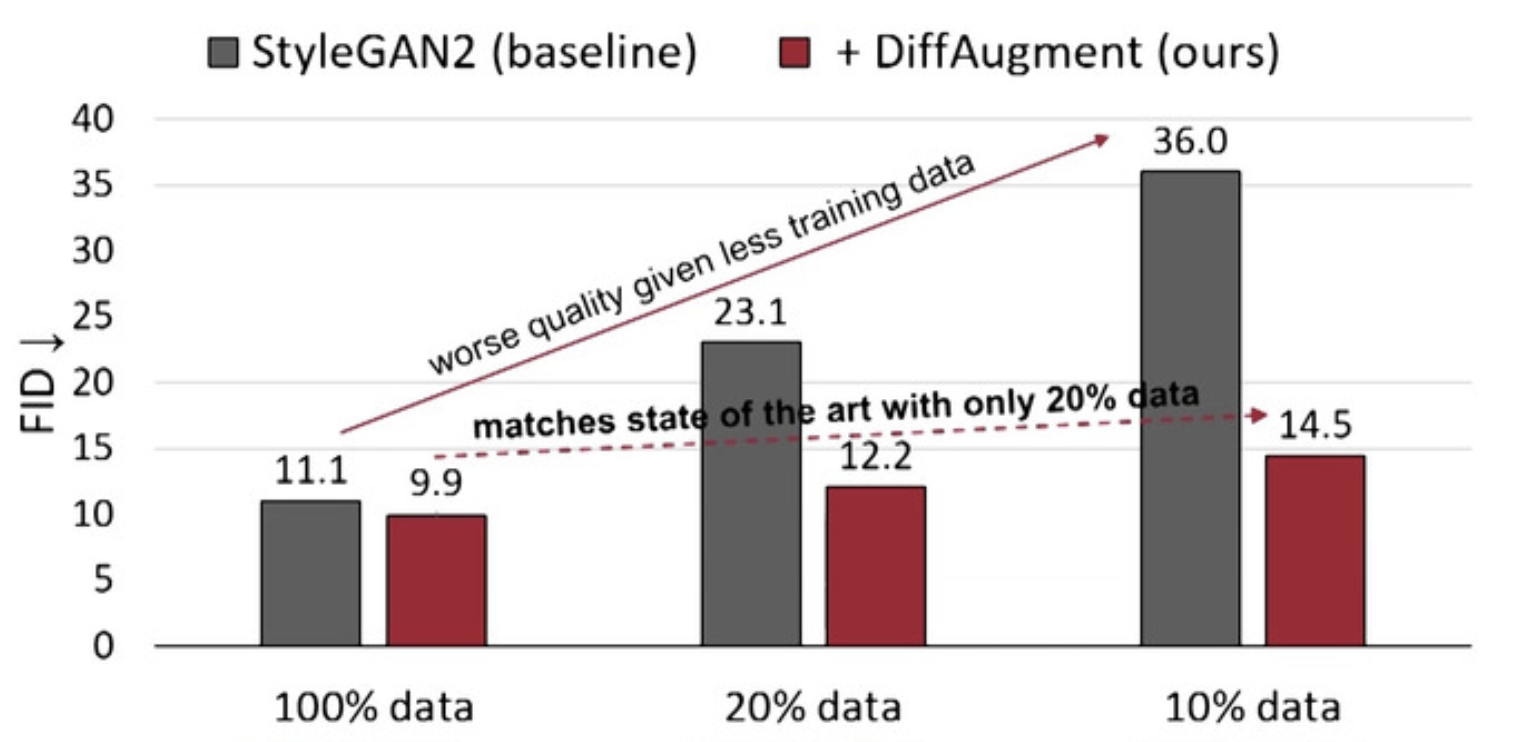
\includegraphics[scale=0.4]{neurips-2020/images/Screenshot 2020-12-11 at 10.43.05.png}
    \caption{Illustration of advantages of using differentiable augmentation on when size of available dataset is limited. Gray bins represent FID scores for GAN trained without augmentations, red bins represent the same baseline model but trained using differential augmentations.}
    \label{fig:diff_aug_fid}
\end{figure}

{\bf Key takeaways:} differentiable augmentations is in general a great idea, which is extremely useful in practice (proven by lots of independent experiments) for training GANs and other frameworks. Also code is released \href{https://github.com/mit-han-lab/data-efficient-gans}{on GitHub}.

\subsubsection{Bootstrap Your Own Latent - A New Approach to Self-Supervised Learning \cite{GrillSATRBDPGAP20}}

Presented by \textit{Jean-Bastien Grill} (also oral at the Track 27 - Unsupervised/Probabilistic)  \\

{\bf Motivation:} improve self-supervised pretraining of CNNs to provide better initialization for further fine-tuning on the end task. \\

{\bf Observation:} model can be trained not using labels from the training set. Instead, they can be generated by the network itself (its replica), which will allow to train without negative labels (potentially better performance). \\

{\bf Method:} the main features of the method are illustrated on figure \ref{fig:self_supervision_framework}.

\begin{figure}[h!]
    \centering
    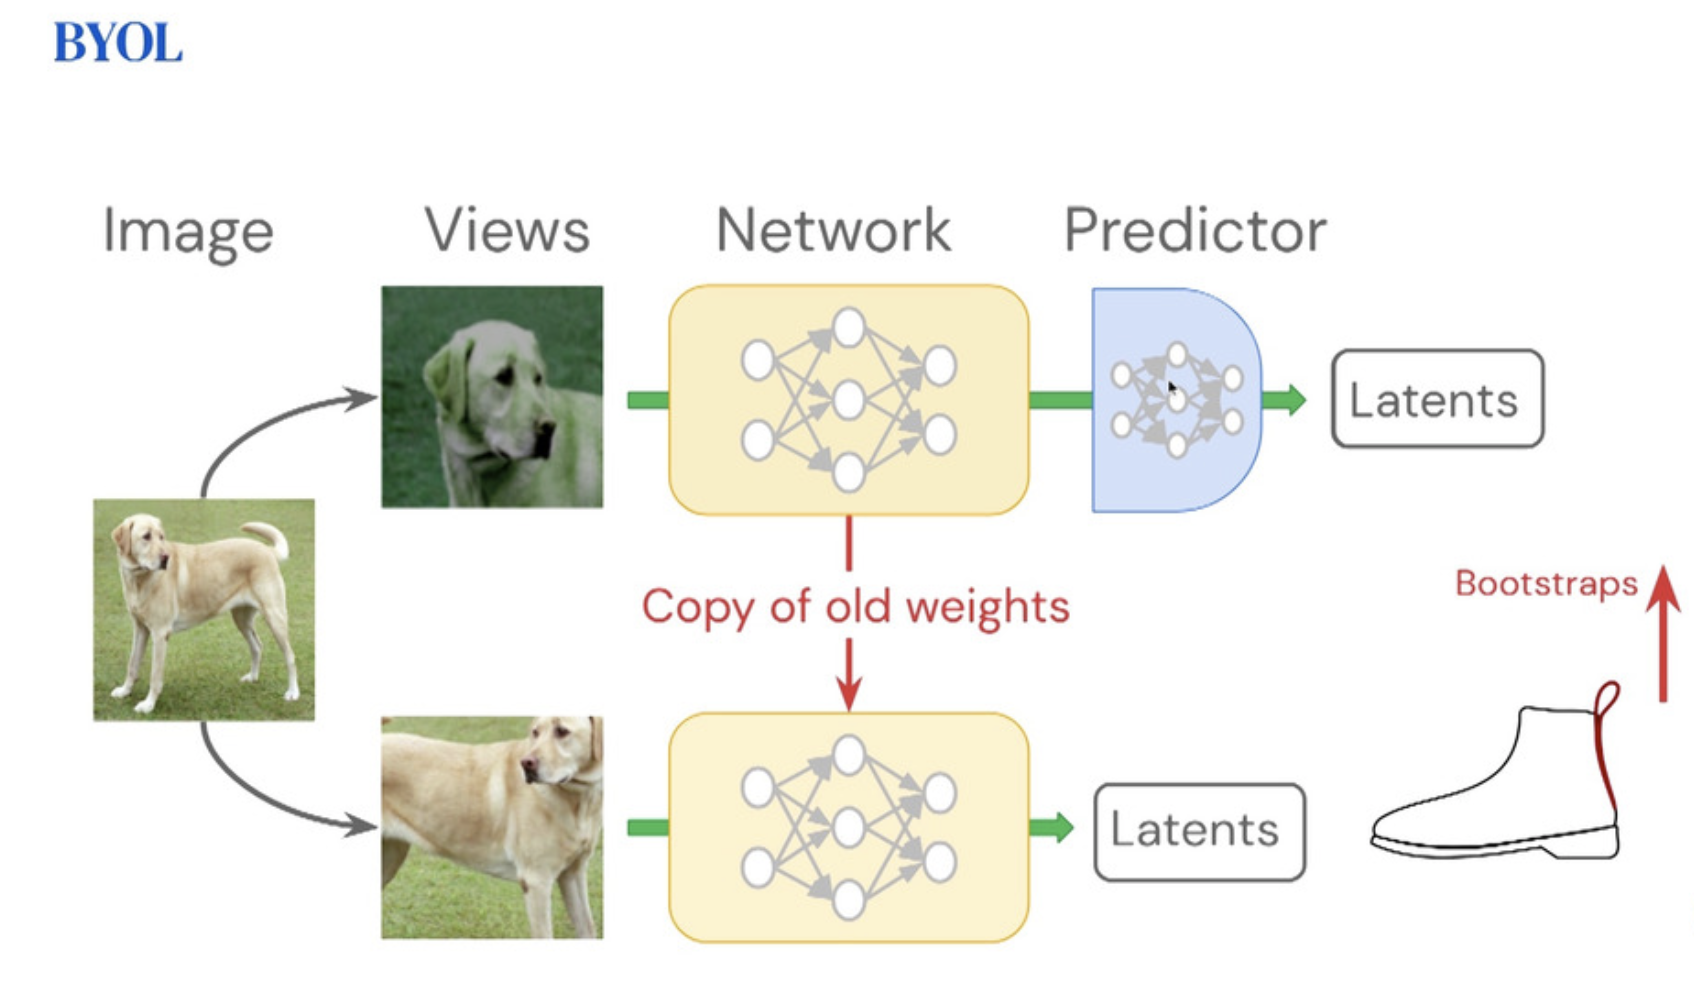
\includegraphics[scale=0.4]{neurips-2020/images/Screenshot 2020-12-11 at 19.06.09.png}
    \caption{Main elements of the BYOL method. First, two different views are extracted from an image from the training set. Second, on the views is fed into the feature extractor and next to the predictor. The predictor outputs latents, which should match bootstrapped outputs of feature extractor replica.}
    \label{fig:self_supervision_framework}
\end{figure} \\

There are several key ingredient of this method:
\begin{itemize}
    \item Carefully tuned image transformations
    \item Presence of the target network (inspired by Reinforcement Learning)
    \item Additional predictor on online network (makes training more stable)
\end{itemize} \\

{\bf Results:} current SOTA, more resilient to transformation and batch size than contrastive methods. \\

{\bf Key takeaways:} need to try self-supervision in other tasks (may be start with a simpler method). Code is \href{https://github.com/lucidrains/byol-pytorch}{released on GitHub}. \\



\subsubsection{Noise2Same: Optimizing A Self-Supervised Bound for Image Denoising \cite{XieWJ20}}

Presented by \textit{Yaochen Xie}  \\

{\bf Motivation:} enhance previous SOTA self-supervided denoising model Noise2Self \cite{BatsonR19} by solving its main problem - utilization of information about center pixel without knowing the noise model. \\

{\bf Related work:} Noise2Noise \cite{LehtinenMHLKAA18} compared to the proposed approach requires more supervision with noisy-noisy pairs. Here, only unpaired noisy images are available. In Noise2Void \cite{KrullBJ19} and Noise2Self \cite{BatsonR19} \textbf{blind spot denosing} is proposed. Here, some masks are applied and then each pixel is denoised with this context. The biggest disadvantage of this approach is that only surrounding pixel are utilized while the information from the pixel being denoised is not used. This leads to lower performance. Some methods to address it were proposed by they rely on noise model, which is unknown in most cases. \\

{\bf Observation}: one term in the loss function of the Noise2Self model can be bound to be zero instead of assuming it. \\

{\bf Method:} in general, method follows the Noise2Self framework. The only difference is the objecting function. It is changed to meet zero-value requirement instead of assuming it. \\

\begin{figure}[h!]
    \centering
    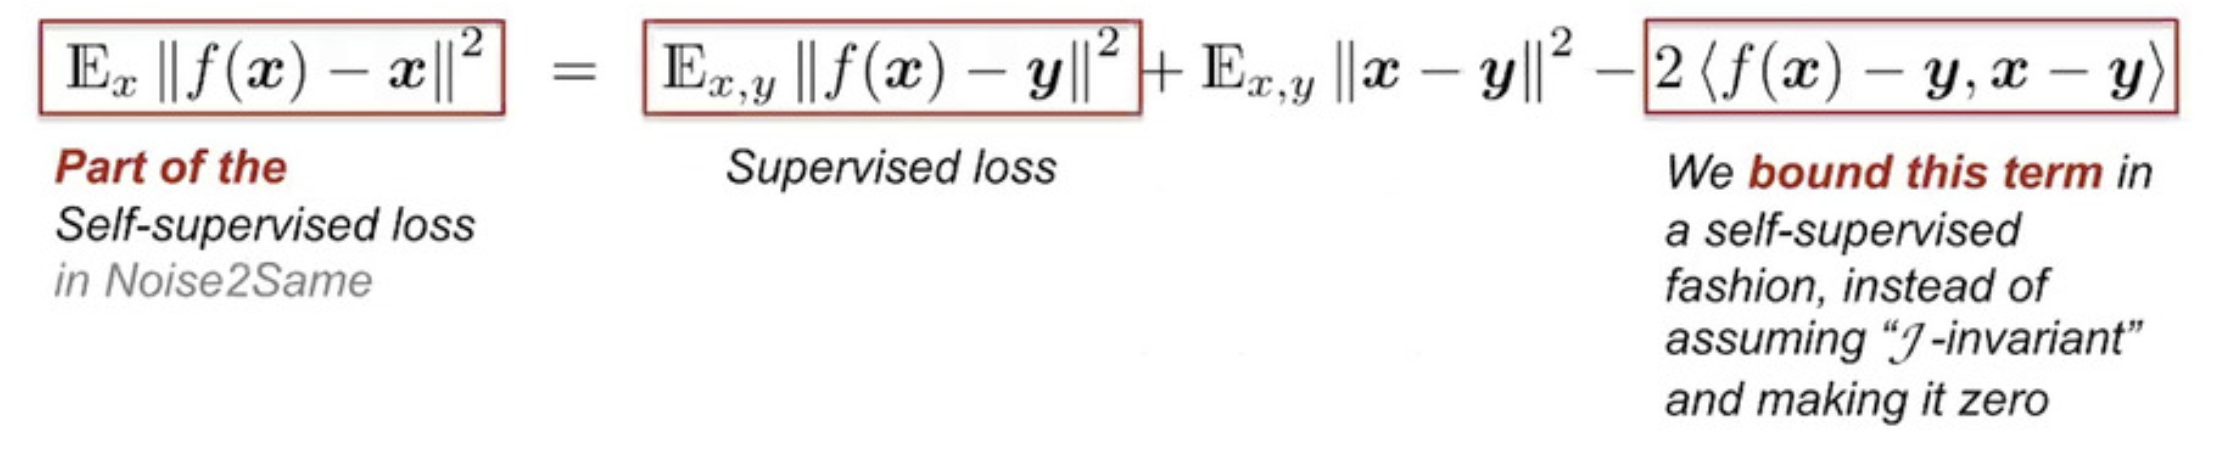
\includegraphics[scale=0.4]{neurips-2020/images/Screenshot 2020-12-12 at 14.58.30.png}
\end{figure} \\

{\bf Results and takeaways:} SOTA results compared to other self-supervised/weakly supervised methods, code is \href{https://github.com/divelab/Noise2Same}{released on GitHub}. \\




\subsubsection{3D Self-Supervised Methods for Medical Imaging \cite{TalebLDSGBL20}}

Presented by \textit{Aiham Taleb}  \\

{\bf Motivation:} most of known self-supervised method are developed for 2D data. However, there is a way to utilize 3D spacial information, which is often available in medical imaging. \\

{\bf Method:} adapt 2D self-supervied pretraining methods to 3D. The following methods are adapted:
\begin{itemize}
    \item Contrastive Predictive Coding
    \item Rotation Prediction
    \item Relative Patch Location
    \item Jigsaw Puzzle Solving
    \item Exemplar Networks
\end{itemize} \\

{\bf Results and takeaways:} not much novelty but code for the proposed 3D methods is \href{https://github.com/HealthML/self-supervised-3d-tasks}{released on GitHub}. \\